\documentclass[12pt]{article}

\usepackage[left=0.9in,right=0.9in,top=0.8in,bottom=1.05in]{geometry}
\newcommand{\ligne}[1]{\rule[0.5ex]{\textwidth}{#1}\\}

\usepackage[]{graphicx}
\usepackage{wrapfig}
\usepackage{physics}
\usepackage{color}
\usepackage{amsthm}

\definecolor{coloradoRed}{rgb}{0.80,0.27,0.16}

\usepackage[breakable]{tcolorbox}
\usepackage{graphicx}
\usepackage{enumitem}

\NewDocumentEnvironment{solution}{O{} O{no}}
{
    \begin{tcolorbox}[
        breakable,
        colback=white,
        colframe=black,
        boxrule=0.5pt,
        arc=0pt,
    ]
    \begin{minipage}{\linewidth}

    \textcolor{coloradoRed}{\textbf{Result:}}\par\noindent

    \ifstrequal{#2}{yes}{
        \begin{enumerate}[label=(\alph*)]
            \item 
            \mbox{}\par
    }{}

    \if\relax\detokenize{#1}\relax
        % No image argument -- do nothing
    \else
        
            \centering
            \includegraphics[width=1.0\linewidth]{#1}
       
    \fi

    \ifstrequal{#2}{yes}{
        \end{enumerate}
    }{}

    \end{minipage}
}
{
    \end{tcolorbox}
}
% \newenvironment{proof}
% {\par\noindent\textit{Proof.}}
% {\hfill\qed\par}

\begin{document}

\begin{flushleft}
    \textbf{Department of Applied Mathematics and Statistics} \\
    \textbf{COLORADO SCHOOL OF MINES} \\
    Math $550$: Numerical Solutions of Partial Differential Equations \\
    Charles Girard

\end{flushleft}


\begin{center}
\bf{Numerical PDEs Homework \#1}\\
\bf{Due Tuesday October 6, 2026}
\end{center}

\vspace{0.3cm}

\noindent \textbf{Problem 1: Solve the Stokes Equations}
For the Stokes Equations in 2D:
$$
\begin{aligned}
    \mu \nabla^2 \mathbf{u} - \nabla p = \mathbf{f}, \quad \nabla \cdot \mathbf{u} = 0,
\end{aligned}
$$
\begin{enumerate}[label = (\alph*)]
    \item Explain why the boundary conditions for $P$ are not necessary on the top and bottom boundaries, yet are for the periodic (left and right) boundaries.
    \item Solve Stokes for the analytical solution:
        $$ \begin{aligned}
            U_{an}(x,y) &= \sin(2\pi y) \sin(2 \pi x), \\
            V_{an}(x,y) &= -3.5 + \cos(2\pi x)\left[ \cos(s\pi y) - 1 \right], \\
            P_{an}(x,y) &= \sin(2\pi y) \cos(\pi x), 
        \end{aligned} $$
        with the corresponding boundary conditions:
        $$  \begin{aligned}
            &\text{Periodic boundary conditions on the left and right boundaries: }\\ &\quad u(0,y) = u(1,y), \quad v(0,y) = v(1,y), \quad p(0,y) = p(1,y) \\
            &\text{Dirichlet (no-slip) boundary conditions on the top and bottom boundaries for $U$: } \\ &\quad u(x,0) = u(x,1) = 0, \\
            &\text{Dirichlet (inflow/outflow) boundary conditions on the top and bottom boundaries for $V$: } \\ &\quad v(x,0) = v(x,1) = -3.5.
        \end{aligned} $$
\end{enumerate}

\begin{solution} \begin{enumerate}[label=(\alph*)]
    \item As one is often encouraged to remember, $P$ is not a value that is directly prescribed for the Stokes equations.
     It is much better thought of as a Lagrange multiplier that allows one to enforce the incompressibility condition. 
     Therefore, specifying boundary conditions for $P$ on the top and bottom boundaries is not necessary, while for the periodic boundaries, consistency requires that $P$ matches on both sides.
     Since $P$ will be correct accurate only to a constant, having a specific value for $P$ in mind to solve Stokes is not necessary.
     On the contrary, having a well-defined Dirichlet condition for $P$ on the top and bottom boundaries can over-constrain the problem and lead to inconsistencies with the incompressibility condition.
     Put another way, $P$ should be determined by the flow field and the incompressibility condition, rather than being directly prescribed on the boundaries.
     The periodic condition is an exception because it does not define a boundary insomuch as it connects one side of the domain to the other, requiring consistency of $P$ across the periodic boundaries.
    \item
    \begin{center}
        \mbox{}\par
        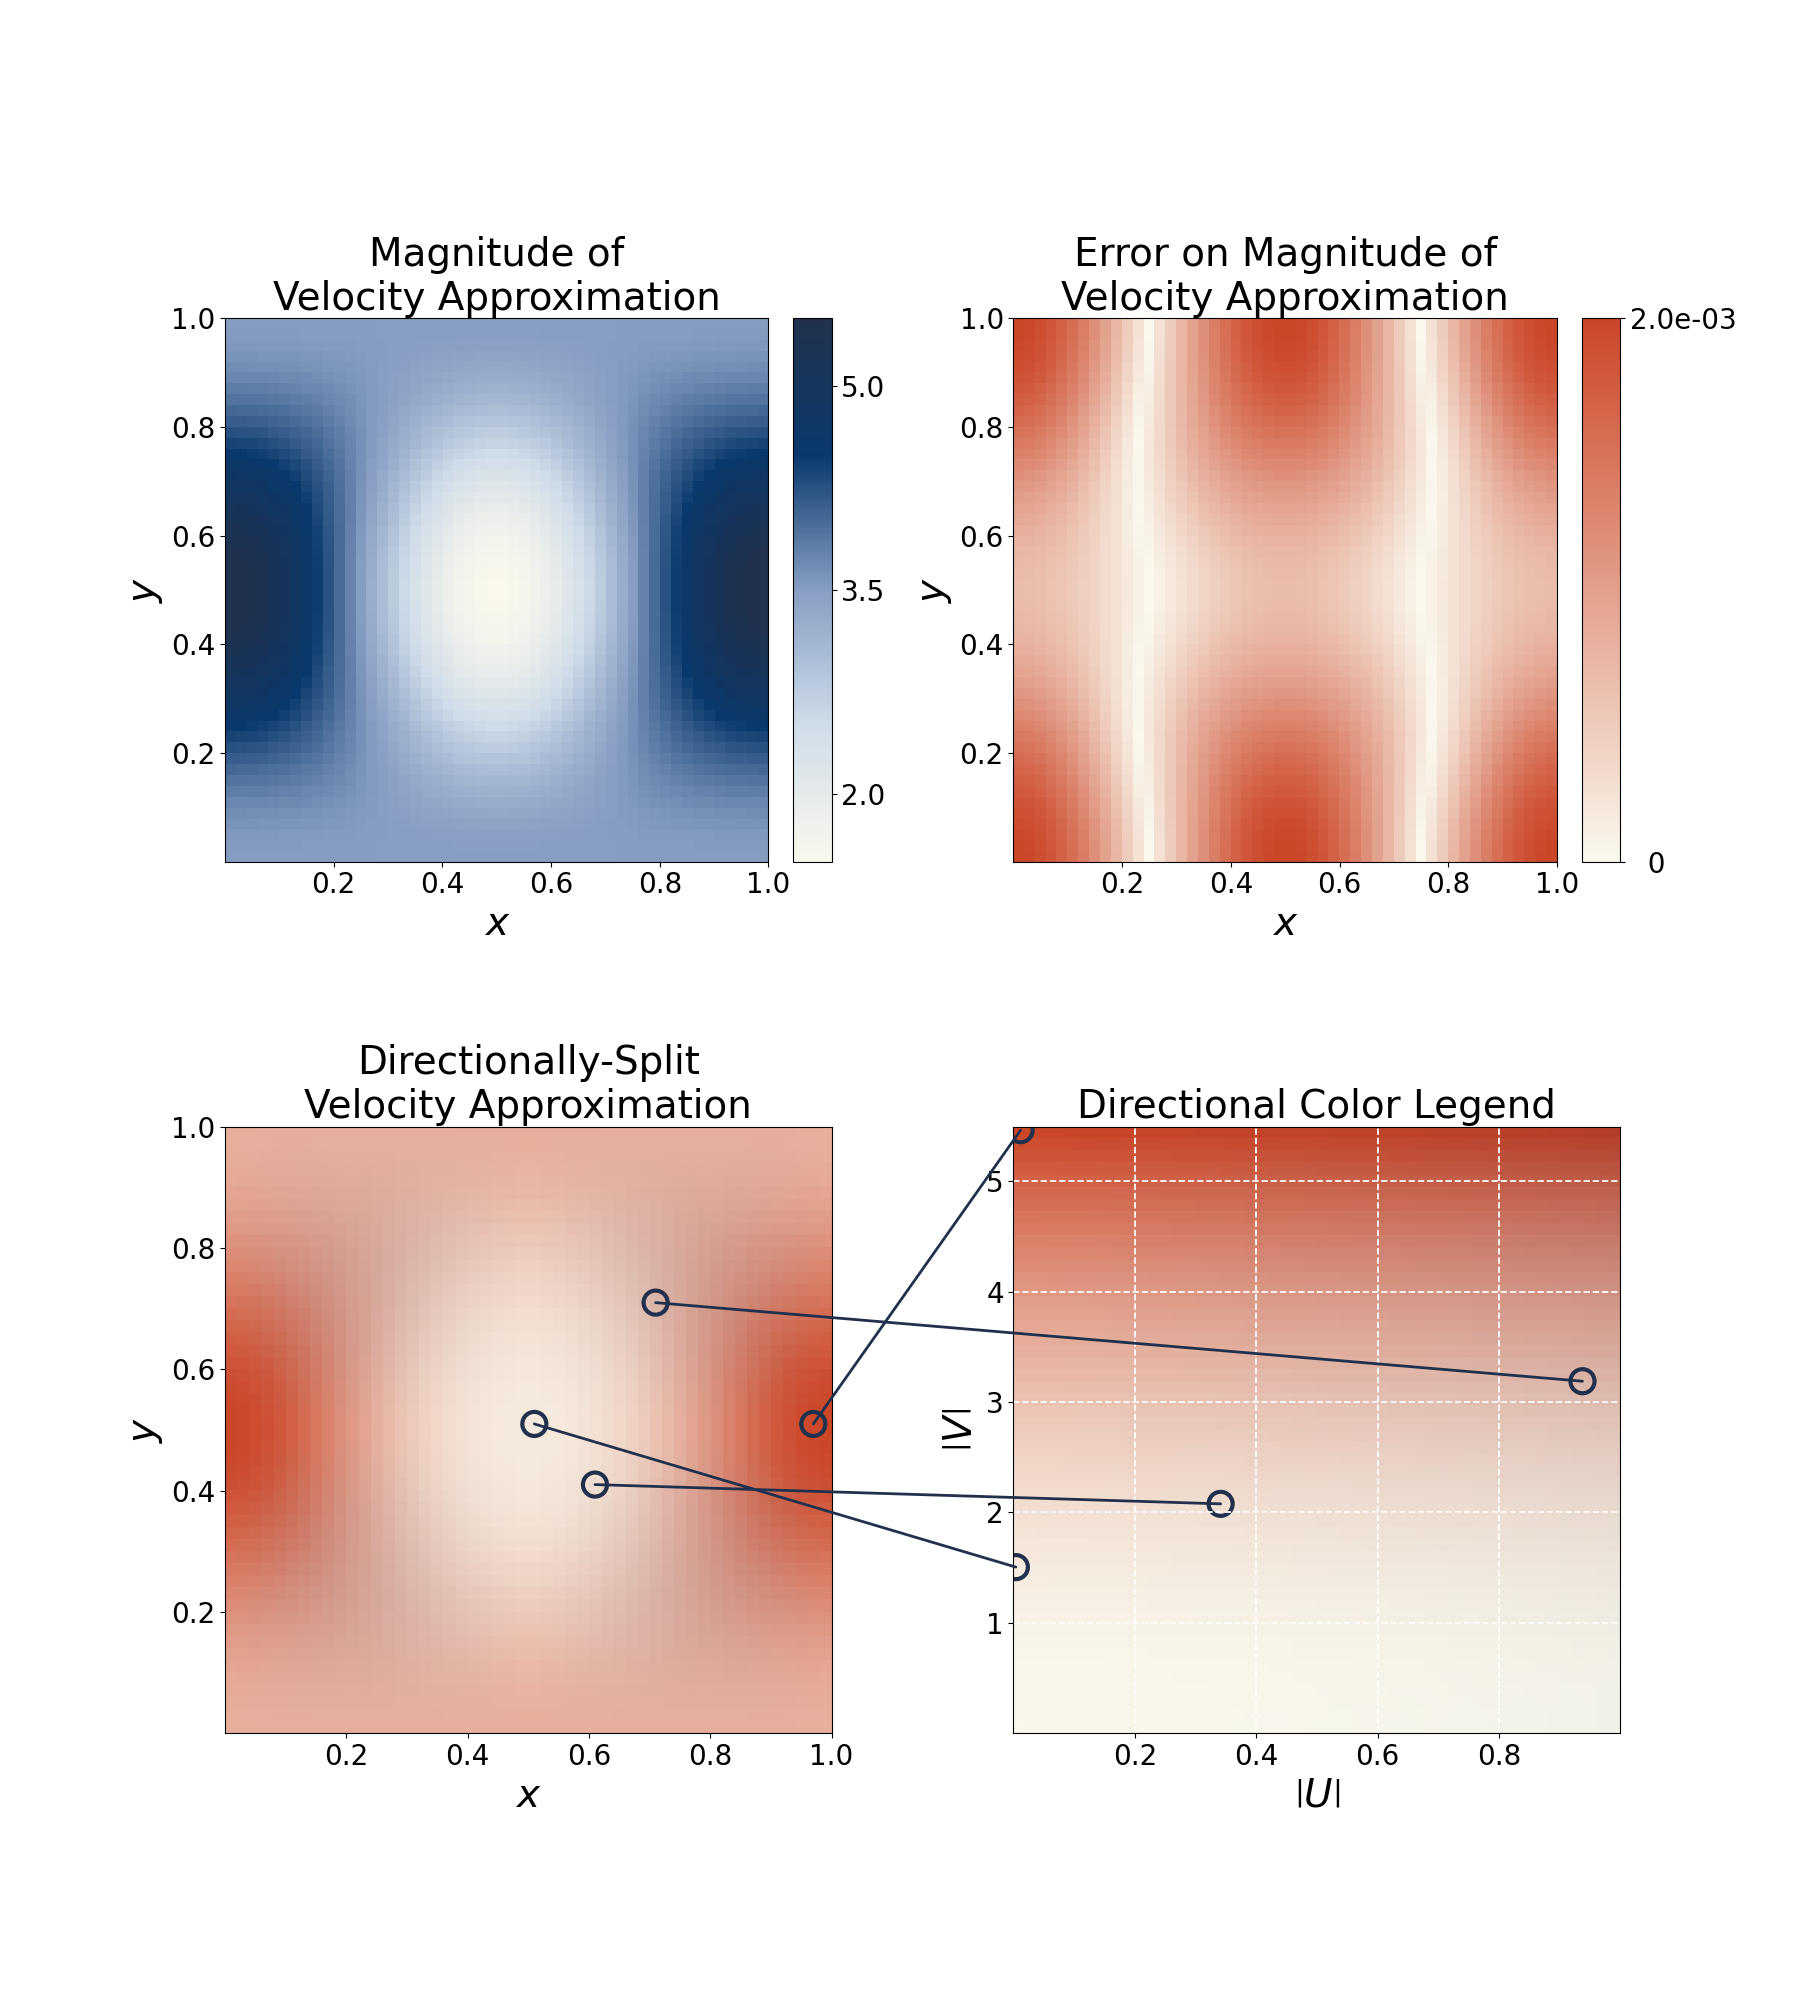
\includegraphics[width=0.95\linewidth]{stokes_plot.png}
        \small Visualization of the Stokes flow field.
        \label{fig:stokes_plot}
    \end{center}
\end{enumerate}
\end{solution}

\vspace{1cm}

\noindent \textbf{Problem 2: Error Analysis}
Define the error of our solution ($\mathbf{u}_{num}$) compared to the analytical solution ($\mathbf{u}_{an}$) as:
$$
\text{err}_\mathbf{u} = \frac{\|\mathbf{u}_{num} - \mathbf{u}_{an}\|_2}{\|\mathbf{u}_{an}\|_2}, \quad
$$
Show that we see second-order error decreases in our numerical solution over an increasing number of grid points ($N_x = N_y = N$).

\begin{solution}
    \begin{center}
        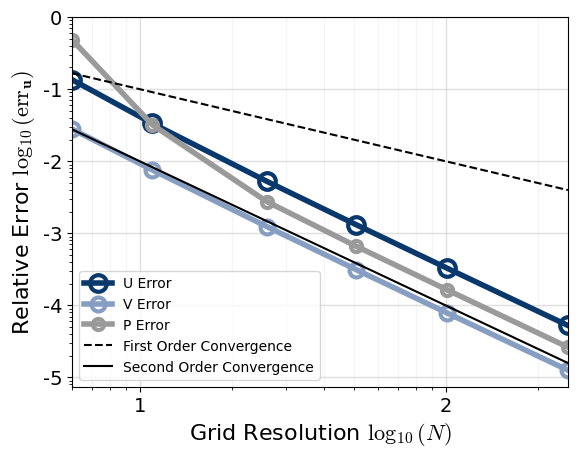
\includegraphics[width=1.0\linewidth]{stokes_error_plot.png}
        \small Error analysis of the Stokes flow numerical solution.
        \label{fig:stokes_error_plot}
    \end{center}
\end{solution}

\vspace{1cm}

\noindent \textbf{Problem 3: Charlie's Fluid Blaster}
Charlie Peskin (the inventor of the IBM) says that you should never just stop once you have a cool code, \textbf{the best part is to play around with it.}
 So do something fun with your code and show it off!

\begin{solution}
    Suppose you devised a way to visualize a flow field in multiple colors based on the direction of the fluid flow, as well as the magnitude of velocity.
    (This was done in problem 1: see Figure \ref{fig:stokes_plot}.)
    However, we have two superficial problems.
    First, the visualization lacks color contrast, because the flow field's velocity is universally biased towards larger $V$ magnitudes.
    For context, the whole field of possible flow field visualization colors that describes \ref{fig:stokes_plot} has much more variety:
    \begin{center}
        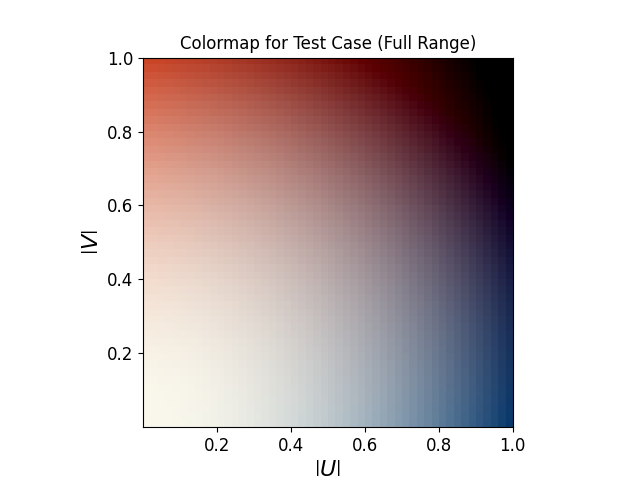
\includegraphics[width=1.0\linewidth]{test_full_colormap.png}
        \small Full colormap visualization of the flow field.
        \label{fig:test_full_colormap}
    \end{center}
    80\% of the colormap range is not utilized in the visualization of \ref{fig:stokes_plot}.
    \\ \\
    Secondly, the image generated, even with more vibrance, still doesn't \(to me\) convey much artistic appeal. 
    Experimenting with normalization of $U$ and $V$ components can provide more contrast at the cost of misinterpreting the relative magnitudes of the velocity components:
    \begin{center}
        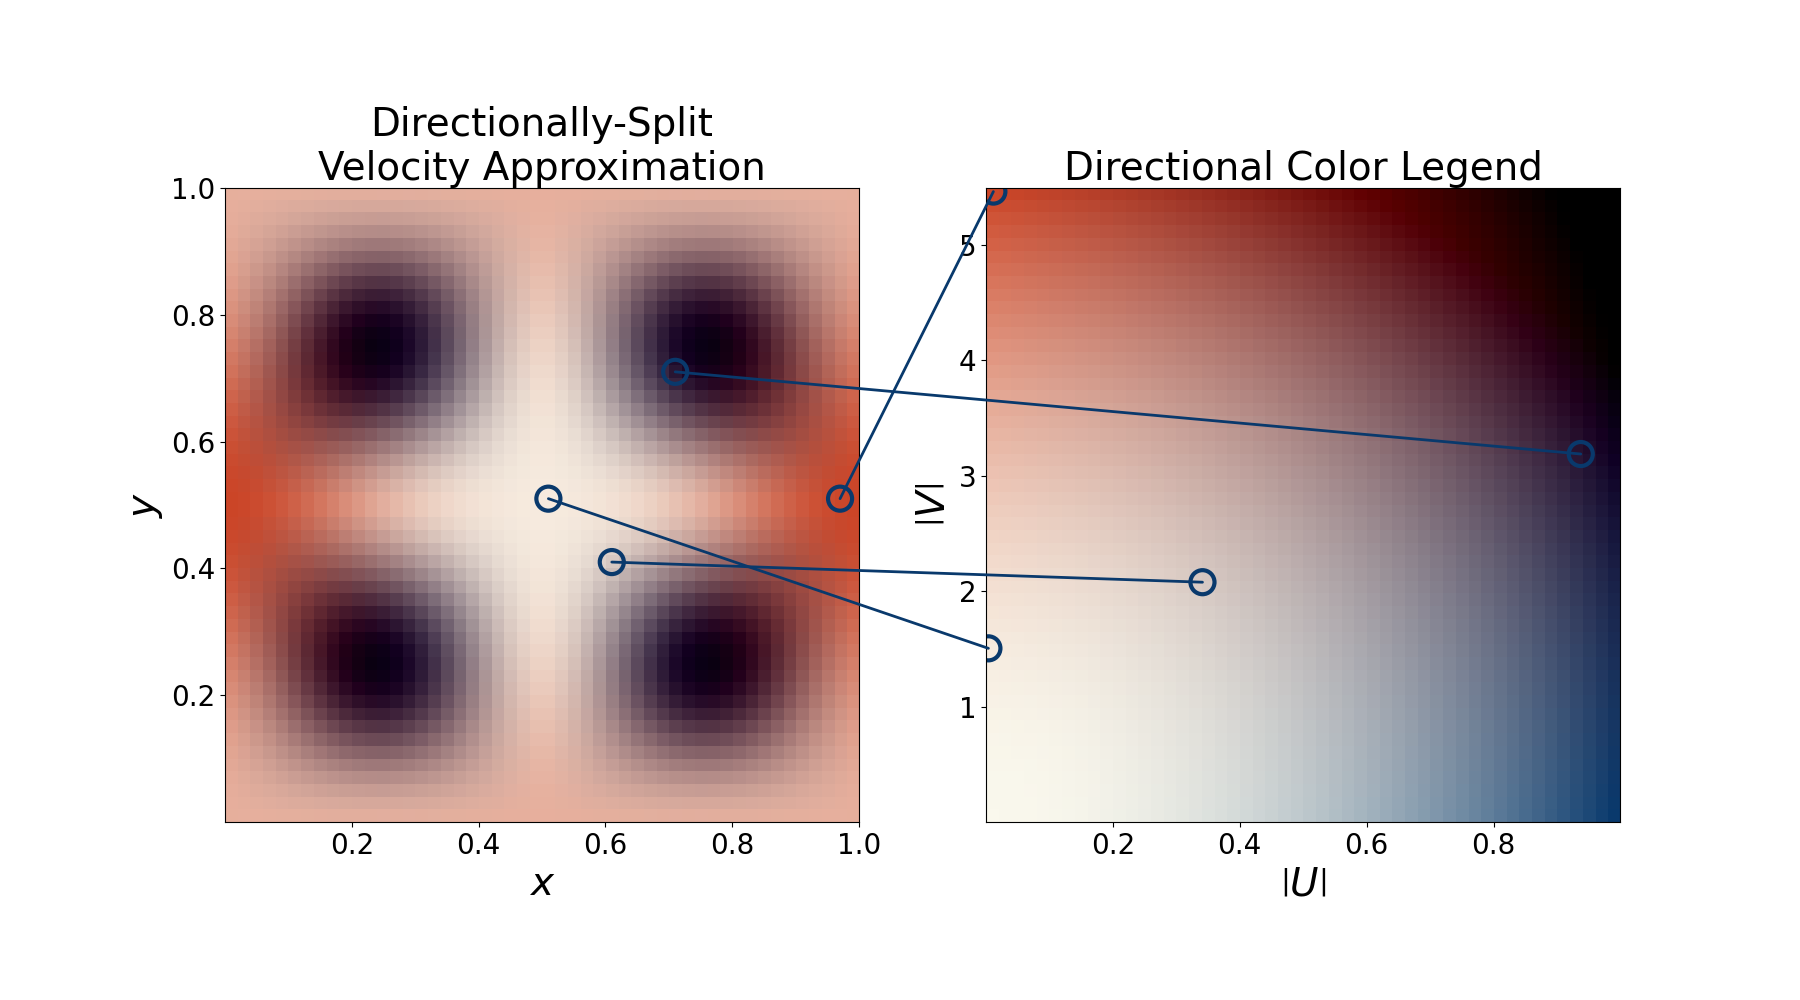
\includegraphics[width=1.0\linewidth]{stokes_plot_better_hues.png}
        \small Enhanced visualization of the Stokes flow field with better color contrast.
        \label{fig:stokes_plot_better_hues}
    \end{center}
    Admittedly, this is cool. But can we do better? Make cooler? \\
    Like Dan Flashes, what if we made it more visually striking?\\
    We've played around with ways to express the analytical solution for long enough.\\
    It's time to do more. New data makes for better visualizations. \\
    \\ \textbf{Step 1: Get Blaster and pixelize him.}
    \begin{center}
        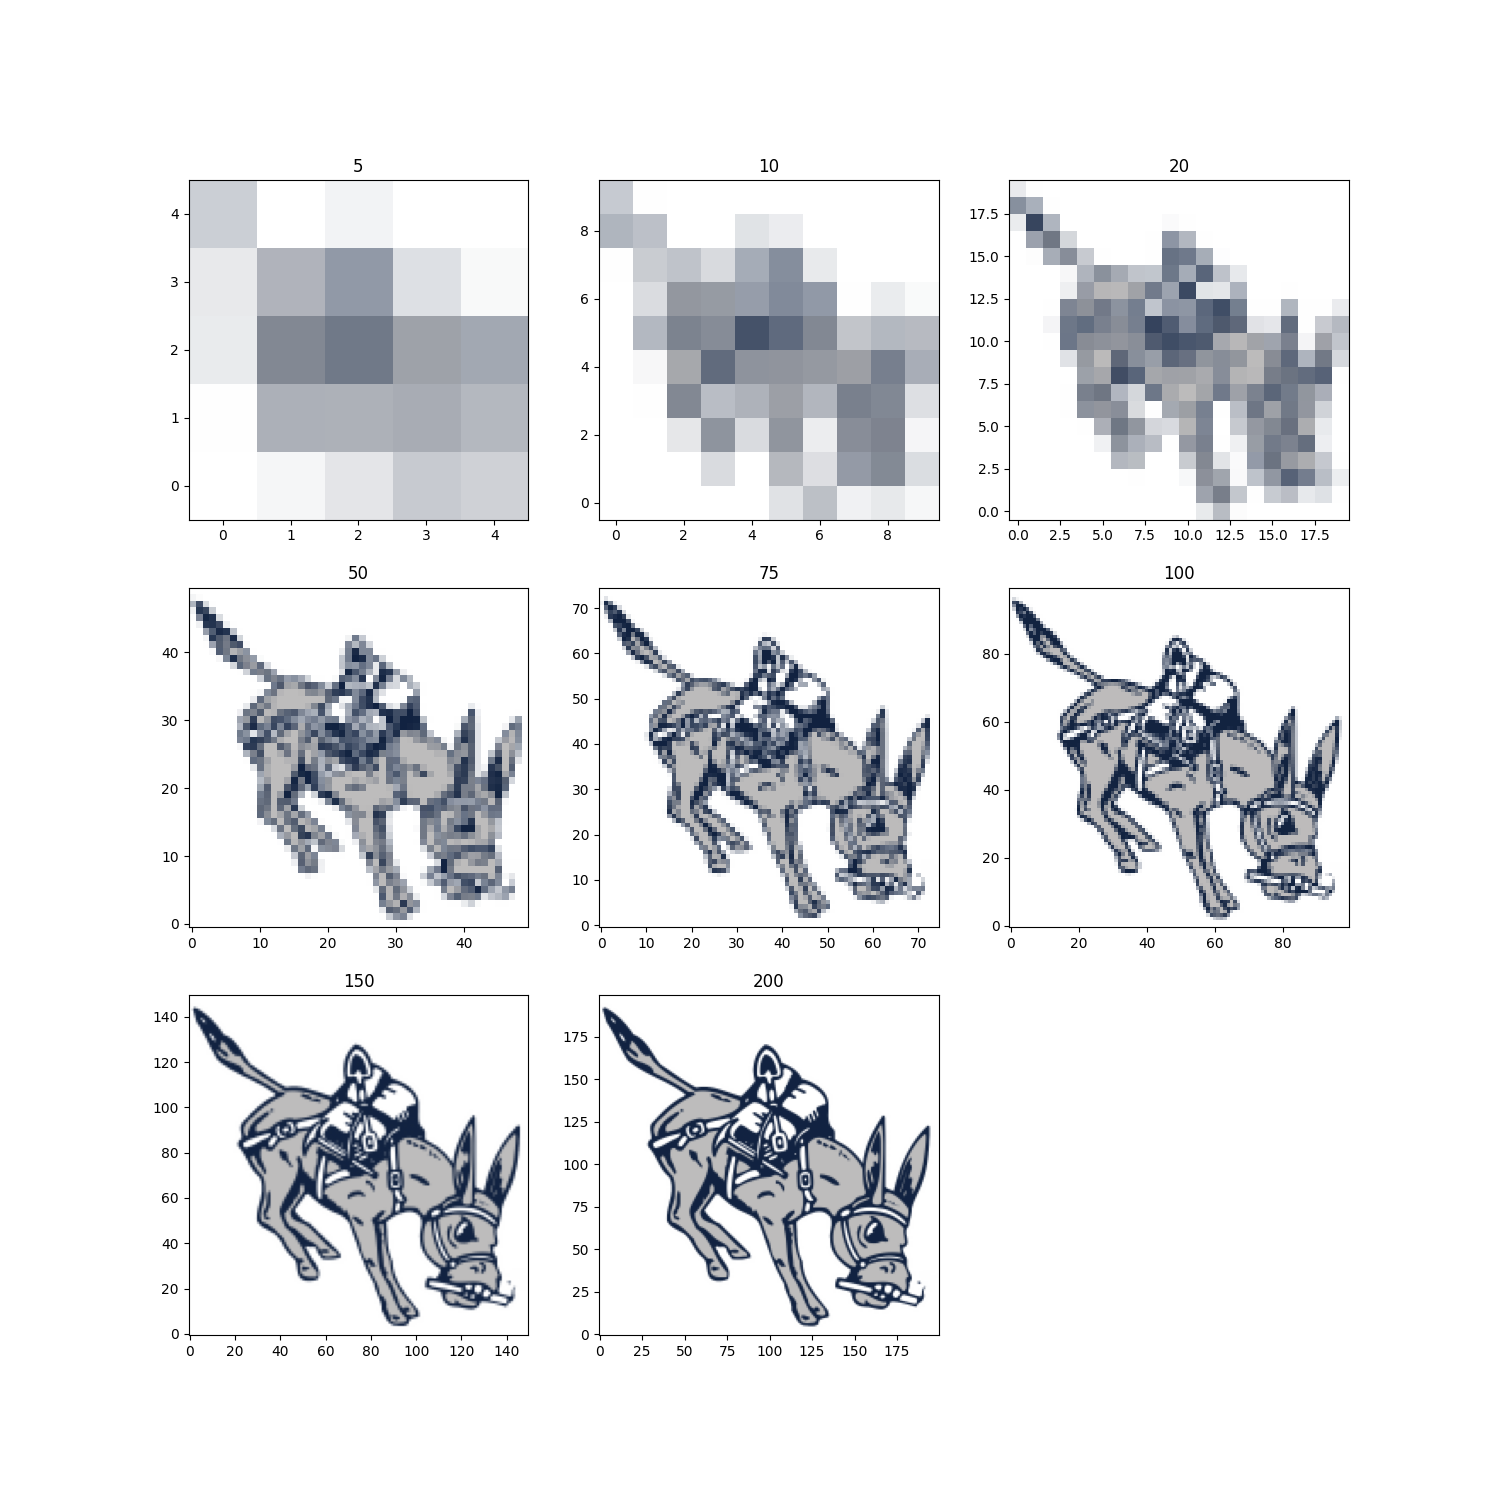
\includegraphics[width=1.0\linewidth]{blaster_pixels.png}
        \small Pixelized version of Blaster.
        \label{fig:blaster_pixelized}
    \end{center}
    \textbf{Step 2: Create a directional colormap for vector fields of the Blaster colors.}
    \begin{center}
        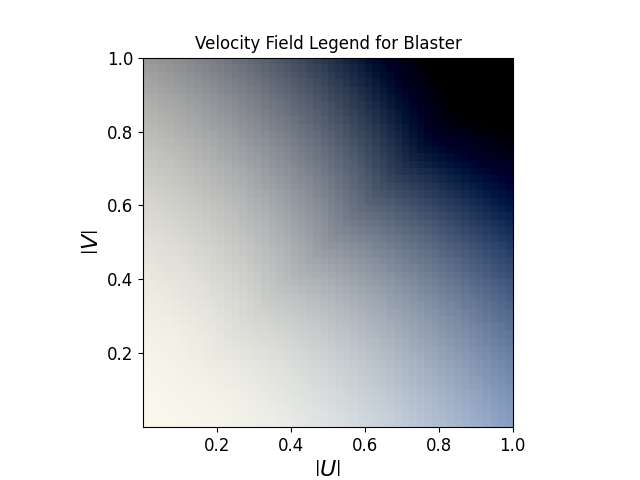
\includegraphics[width=1.0\linewidth]{blaster_colormap.png}
        \small Directional colormap adjusted to Blaster colors.
        \label{fig:blaster_directional_colormap}
    \end{center}
    \textbf{Step 3: Simplify directional colormap to essential colors.}
        \begin{center}
        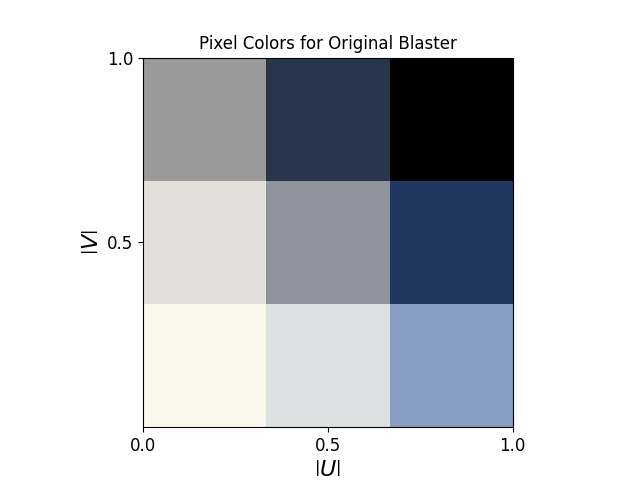
\includegraphics[width=1.0\linewidth]{pixel_colors_original_blaster.png}
        \small Simplified directional colormap to essential Blaster colors.
        \label{fig:pixel_colors_original_blaster}
    \end{center}
    \textbf{Step 4: Project Pixelized Blaster onto the simplified colormap.}
    \begin{center}
        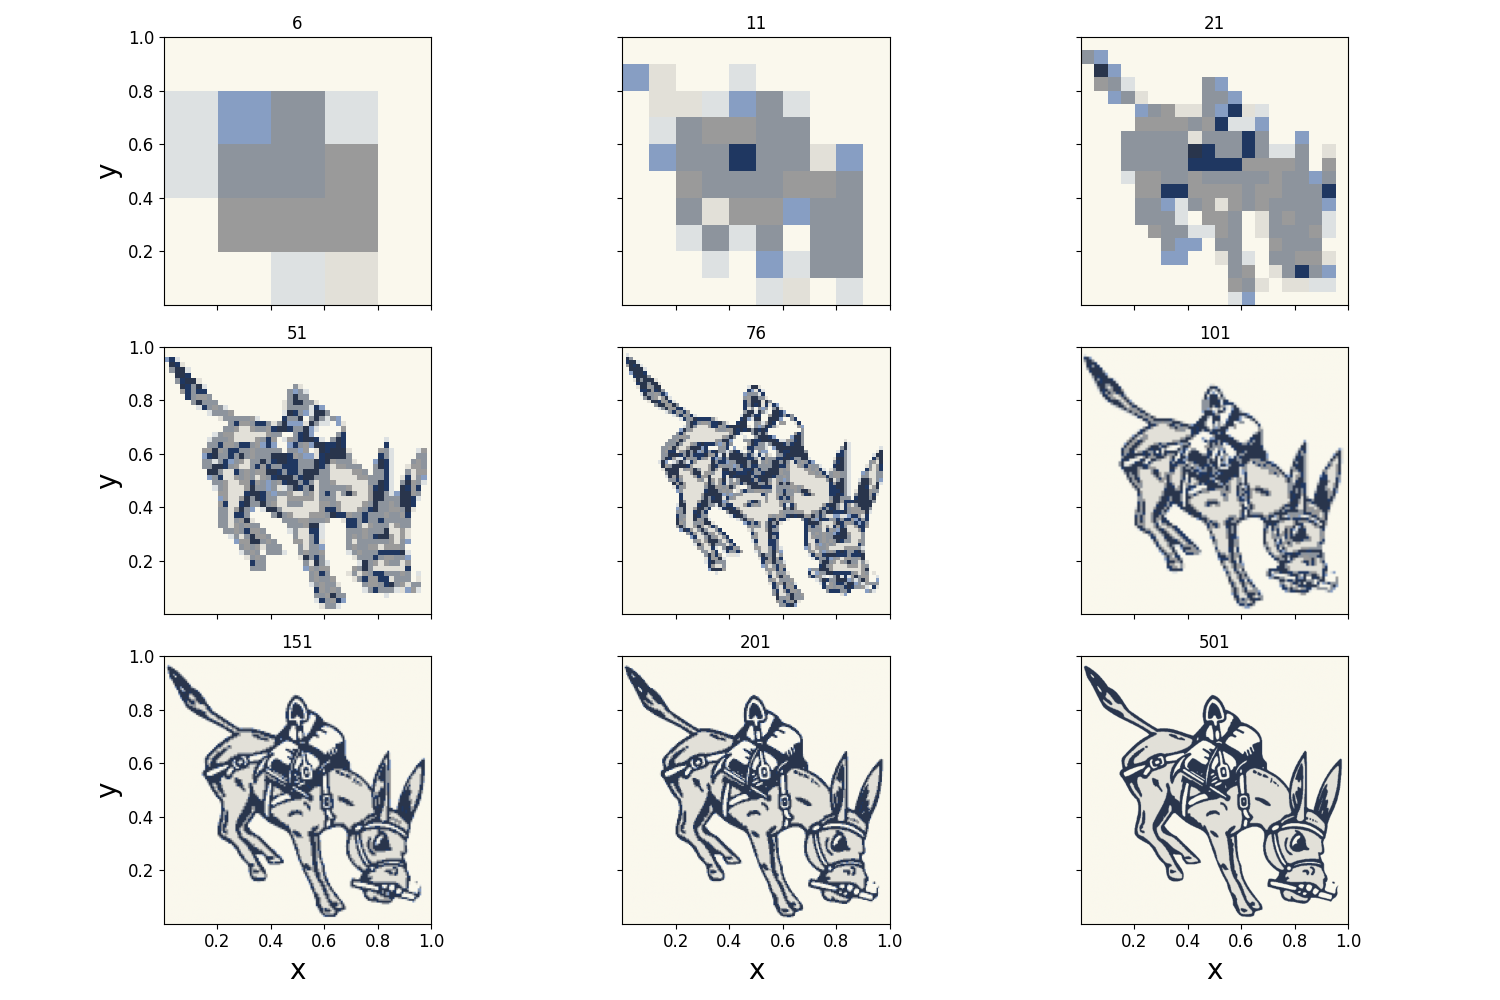
\includegraphics[width=1.0\linewidth]{projected_blaster_colors.png}
        \small Pixelized Blaster projected onto the simplified directional colormap.
        \label{fig:blaster_projected}
    \end{center}
    \textbf{Step 5: Convert Blaster from pixel data to vector field data.}
    \begin{center}
        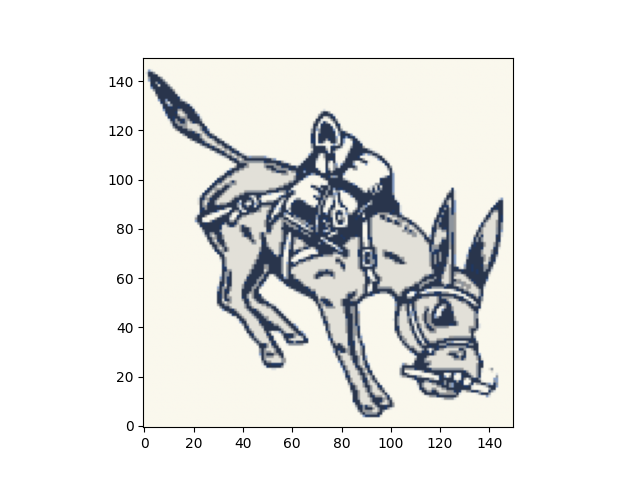
\includegraphics[width=1.0\linewidth]{Vector_Field_Blaster_150.png}
        \small Vector field representation of Blaster derived from pixel data.
        \label{fig:vector_field_blaster}
    \end{center}
    The above figure was generated by mapping \textit{vector Blaster} data through the colormap of Step 3~\ref{fig:blaster_directional_colormap}.
    Blaster is now data indistinguishable from \ref{fig:stokes_plot}.
    However, he's not a fluid yet. Or if he is, he's a very compressable one.
    \\ \textbf{Step 6: Get the Laplacian of Blaster.}
    From our computations for Problem 1, we have a sparse matrix Laplacian operator, which we apply to the Blaster Vector.
    \\ \textbf{Step 7: Solve Stokes to obtain incompressible fluid Blaster}.
    Take the laplacian of Blaster, with 0 as the divergence, as the RHS of the linear system we solved for in Problem 1.
    Adjust the boundary conditions (Dirichlet) such that they match the original (compressible) Blaster vector field.
    The resulting solution will be an incompressible fluid representation of Blaster, preserving the visual characteristics of the original pixelized image.
    \begin{center}
        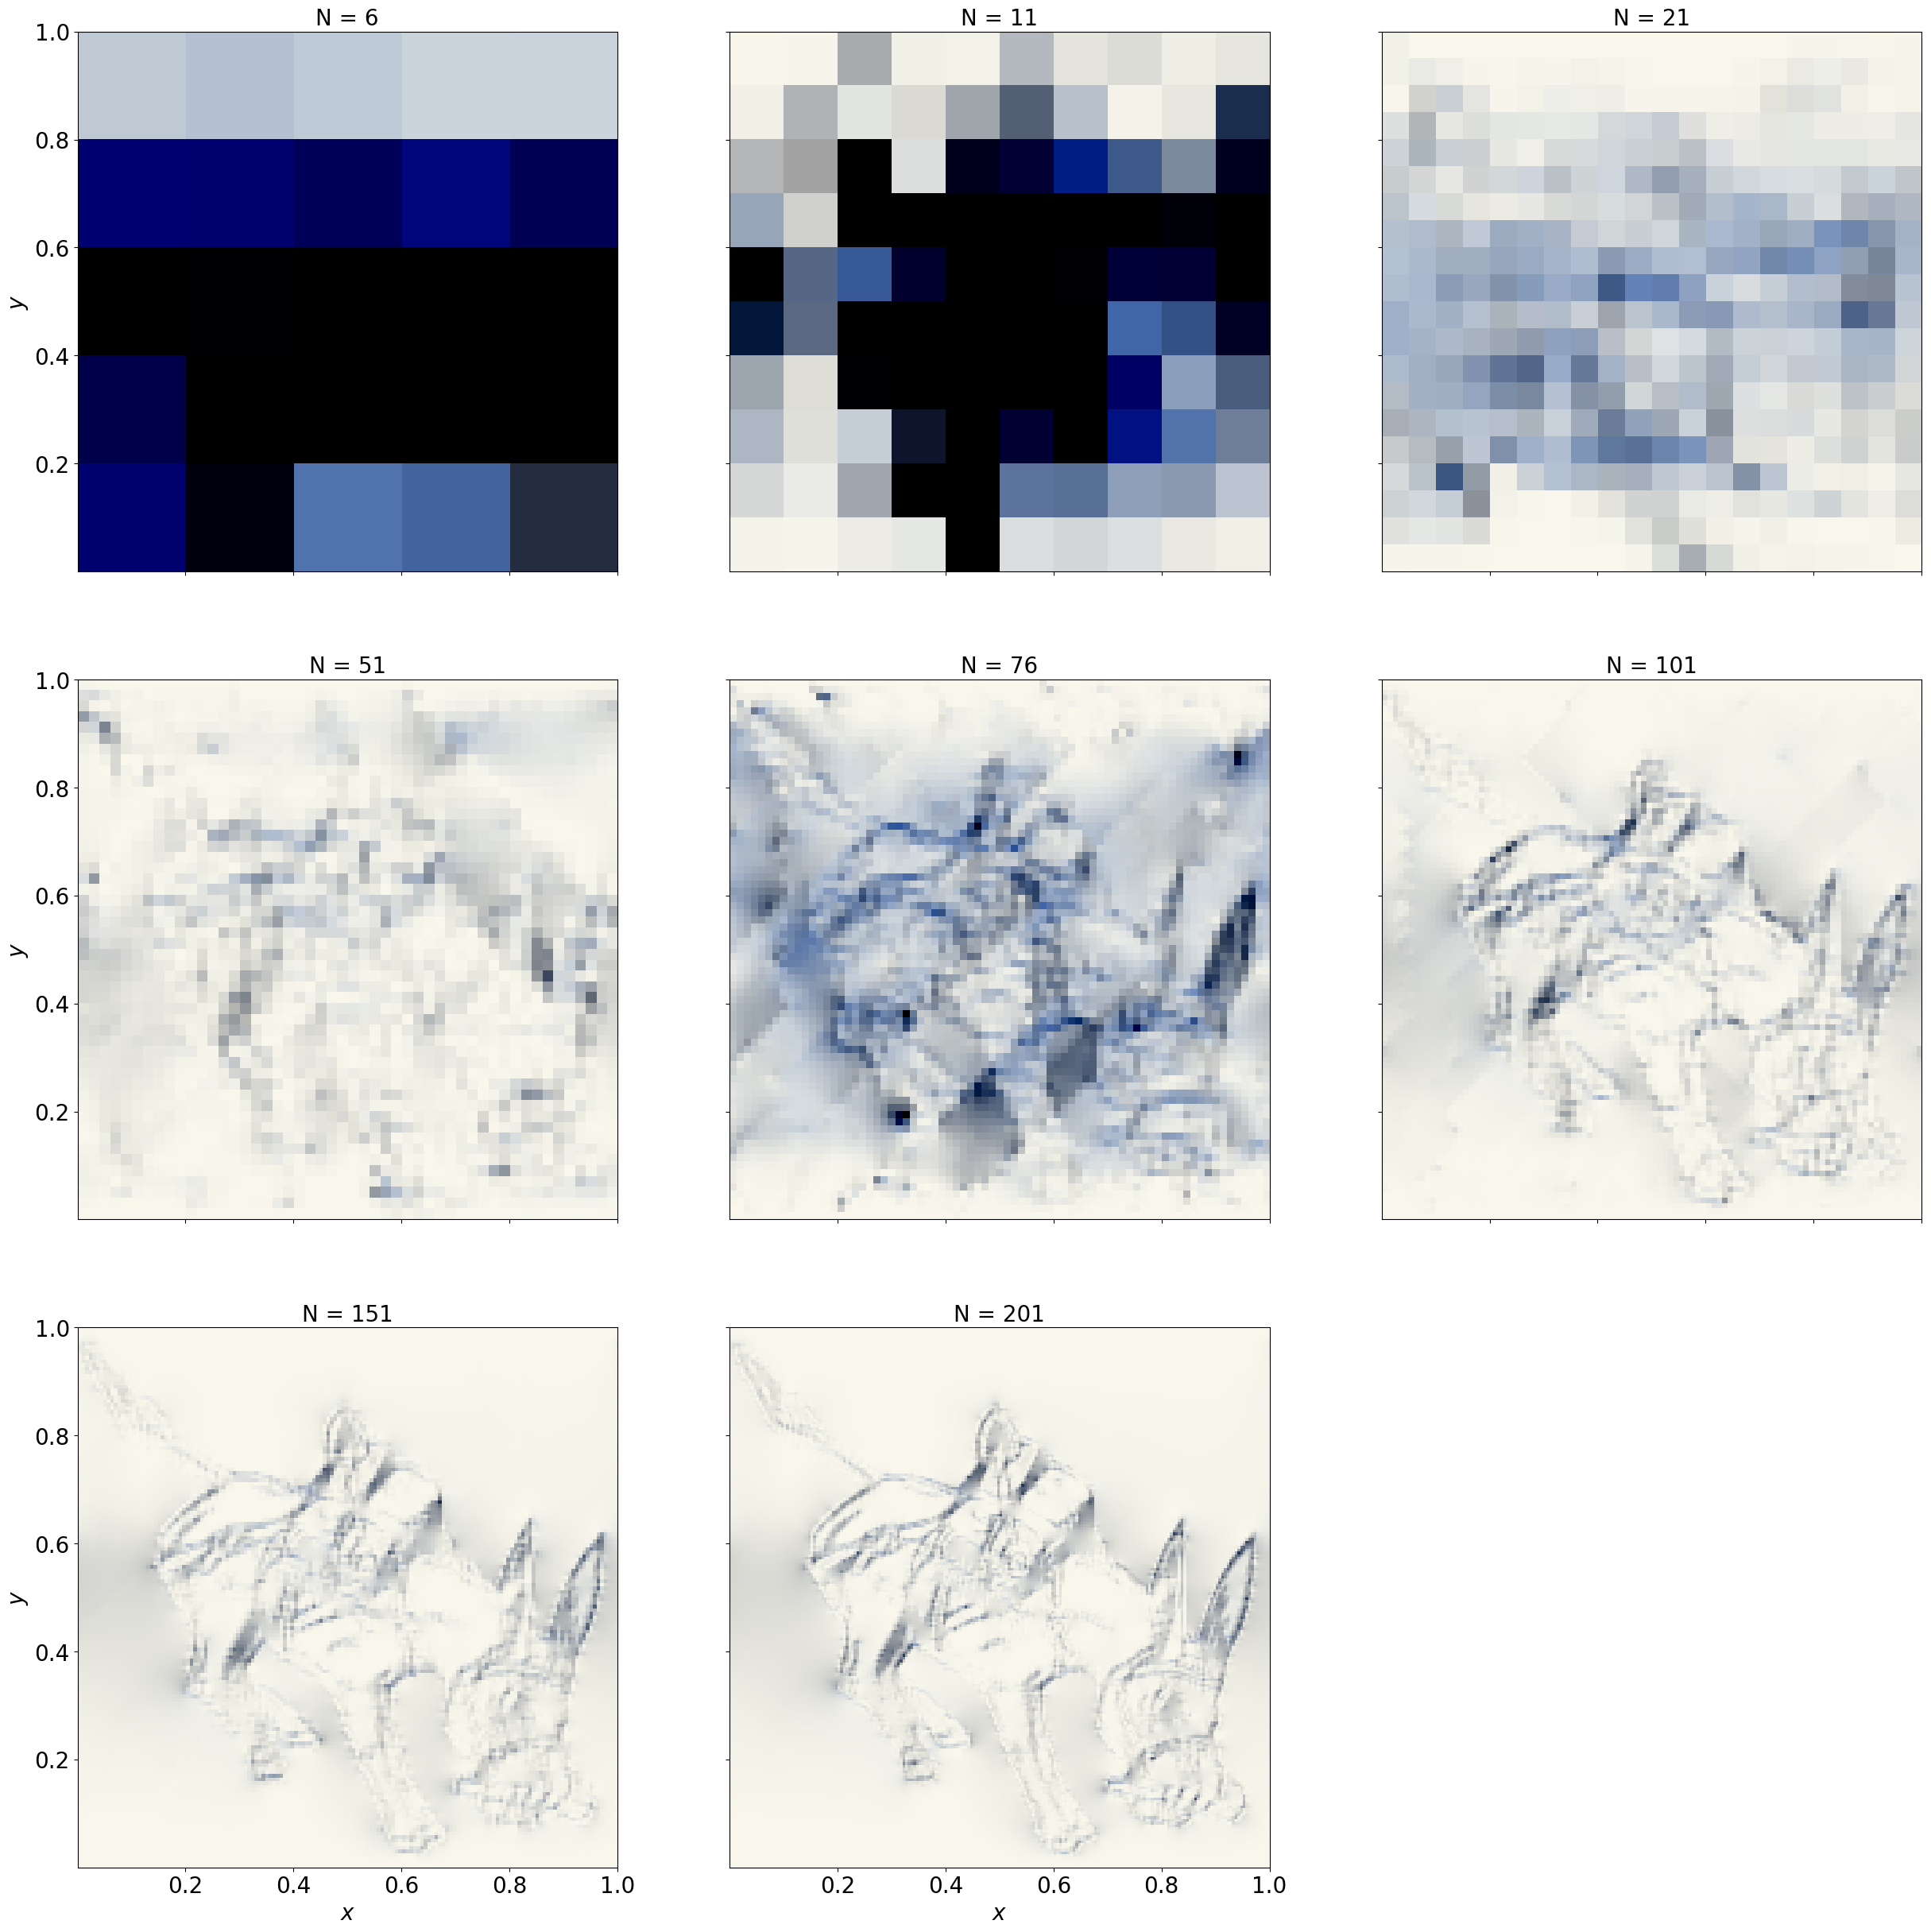
\includegraphics[width=1.0\linewidth]{fluid_blaster.png}
        \small Incompressible fluid representation of Blaster.
        \label{fig:incompressible_fluid_blaster}
    \end{center}
    Future work may involve exploring preservation of the interior silver (High $V$, low $U$) color,
    or mapping 1-norm constrained laplacians to model blaster under operational force-exertion constraints.
\end{solution}
\vspace{0.5cm}

\end{document}